
\subsection{Compléments sur l'analyse temps-fréquence} \label{ann:complement_t-f}

Au delà de permettre de définir les notions d'amplitude et de fréquence instantanée, la transformée en signal analytique viens répondre à un autre problème qu'on les signaux réels pour l'analyse temps-fréquence. 
Aussi, ce problème sera le point de départ de cette annexe pour les introduire la transformée en SA.
Tout le propos portera sur les signaux univariés et est principalement tiré de \cite{cohen_time_1995}.
\\



\subsubsection{Formalisme derrière la transformée en SA ou le problème de signaux réels et comment le résoudre} \label{sec:transfo_SA}

Les notions de densité d'énergie et d'énergie spectrale (\cref{eq:densi_dE}, \Cref{subsec:intro_phased}) :
\begin{align*}
	\densit\ &:\quad \begin{aligned}\R\ &\lr\quad \R^+ \\ t\ &\longmapsto\ \big|x(t)\big|^2 \end{aligned}  
	&
	\text{resp.}\qquad \densis\ &:\quad \begin{aligned}\R\ &\lr\quad \R^+ \\ \nu\ &\longmapsto\ \big|\fou{x}(\nu)\big|^2 \end{aligned}
\end{align*}
sont des concepts centraux en analyse temps-fréquences. Entre autre, leurs moments formalisent les notions de durée d'émission ($\var[\densit]{t}$), de fréquence moyenne ($\esp[\densis]{\nu}$), ou encore de largeur de bande spectrale ($\var[\densis]{\nu}$).
\\

Or, le spectre des signaux réels sont à symétrie hermitienne et leur densité spectrale, $\densis$, symétrique :
\begin{align*}
	\forall t\in\R,\ x(t)\in\R \quad &\Lr \quad \forall \nu\in\R,\ \fou{x}(-\nu) = \congu{\fou{x}(\nu)} \\
	&\Lr \quad \forall \nu\in\R,\ \densis(-\nu) = \densis(\nu)
\end{align*}
\skipl \\
Ainsi, tout signal réel à pour fréquence moyenne 0 et le largeur de bande (variance de $\densis$) est biaisé par la symétrie de $\densis$. 
En plus de ne pas être très instructif, ce n'est pas cohérent avec l'interprétation physique qu'on voudrait avoir de ces objets. Par exemple, si $\densis$ prend la forme ci-dessous (\cref{fig:densi_spec_sym}), alors il serait plus naturelle de demander à ce que la fréquence moyenne se trouve autour de 1,4. De même, la largeur de bande spectrale ne correspond plus à l'étalement de chaque gaussienne, mais plutôt à leur espacement.
\\
\begin{figure}[h]\centering
	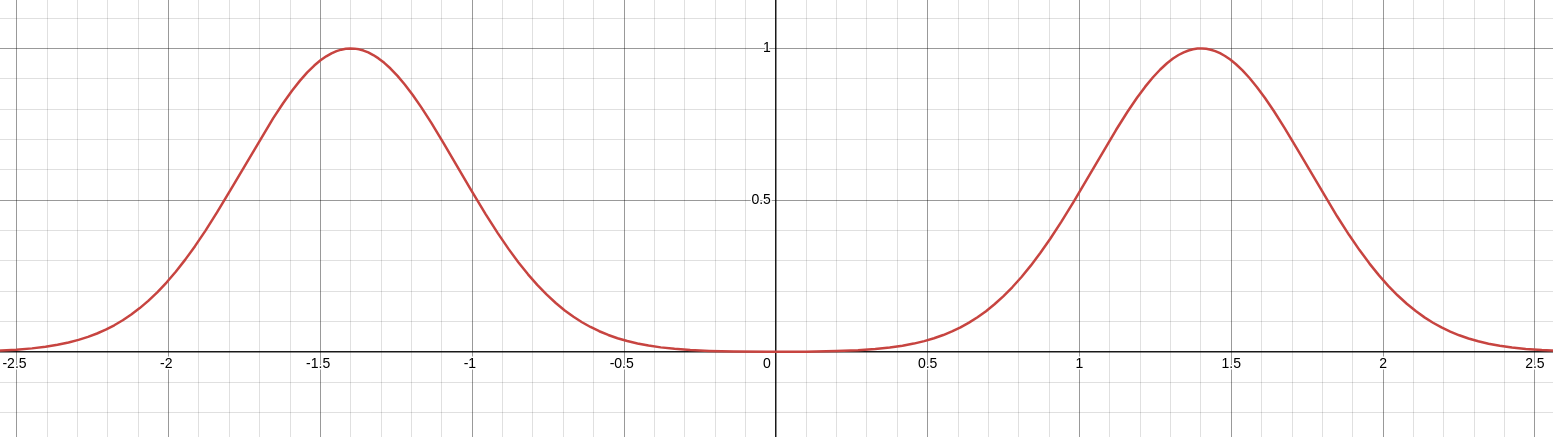
\includegraphics[width=0.9\textwidth]{fig/part-1/densi_spec_sym}
	\caption{\DONE Exemple de densité spectrale d'un signal réel}
	\label{fig:densi_spec_sym}
\end{figure}
\\
Le même problème se pose avec la covariance de $x$. Sachant l'égalité des deux notions de fréquences moyenne (\cref{eq:esp_freq}, \Cref{subsec:intro_phased}) :
\[\esp[\densis]{\nu} = \frac{1}{2\pi}\int_\R \phi'(t)\densit(t)dt = \esp[\densit]{\frac{1}{2\pi} \phi'}\]
\\
on peut définir la covariance temps-fréquence d'un signal $x$ par :
\begin{align*}
	\text{Cov}(x) \defeq \text{Cov}\big(t,\phi'(t) \big) 
	&= \esp[\densit]{t\phi'(t)} - \esp[\densit]{t} \esp[\densit]{\phi'(t)} \\
	&= \esp[\densit]{t\phi'(t)} - \esp[\densit]{t} \esp[\densis]{\nu}	
\end{align*}
\\
Ce coefficient est sensé mesurer une corrélation entre l'évolution d'un signal au cours du temps avec ses fréquences. S'il est réel, alors  $\text{Cov}(x)$ sera toujours nulle mais de là à en conclure que la fréquence instantanée de n'importe quel signal (réel) est toujours décorrélée du temps serait, pour le moins, insatisfaisant.
\\

Pour résoudre le problème, une méthode consiste tout simplement se débarrasser des fréquences négatives du signal, donnant un nouveau signal $\SA{\x}$ :
\begin{align*}
	\Fou{\SA{x}}= 2\one_{\R^+}\fou{x}\ \Lr\ \SA{x} &= 2\iFou{\one_{\R^+}\fou{x}} \\
	&= 2 \iFou{\one_{\R^+}} * x
\end{align*}
\\
où $\one_{\R^+}$ est la fonction indicatrice de $\R^+$ et où le facteur 2 assure la conservation de l'énergie du signal. Cela mène à la définition :
\\
\begin{definition}[Transformée de Hilbert et en SA]\label{def:transfo_sa&hilbert}
	On appelle \emph{transformé de Hilbert de} $x$, l'application :
	\begin{equation}\label{eq:transfo_Hilb}
		\mathcal{H}[x] :\ \begin{aligned} 
			\R \quad &\lr\qquad\quad \C \\	
			t\quad &\longmapsto\ \frac{1}{\pi}\fint_\R \frac{x(s)}{t-s}ds %=  \frac{1}{\pi}\left(\vpC\right)*x
		\end{aligned}
	\end{equation}
	où l'intégrale barrée représente la \emph{valeur principale de Cauchy}, une généralisation aux distributions de la fonction inverse :
	\begin{align*}
		\fint_\R \frac{x(s)}{t-s}ds &\defeq \lim_{\varepsilon\lr0^+} \int_{-\infty}^{-\varepsilon} \frac{\varphi(t)}{t}dt + \int_{+\varepsilon}^{+\infty} \frac{\varphi(t)}{t}dt 
		%\\ &= \int_0^{+\infty} \frac{\varphi(t) - \varphi(-t)}{t}dt
	\end{align*}
	Avec, la \emph{transformée en signal analytique} (SA), alors définie comme l'unique application $\SA{x}$ telle que $\ \Fou{\SA{x}\big.}= 2\one_{\R^+}\fou{x}$, s'écrit explicitement :
	\begin{equation}\label{eq:transfo_SA}
		\SA{x} :\ \begin{aligned} 
			\R \quad &\lr\qquad\quad \C \\	
			t\quad &\longmapsto\ x(t) + i\mathcal{H}[x](t) %= x(t) + \frac{i}{\pi}\fint_\R \frac{x(s)}{t-s}ds
		\end{aligned}
	\end{equation}
\end{definition}
\skipl

Cette transformée permet, à la fois d'avoir un signal propice à une analyse temps-fréquence, et de donner une décomposition canonique $x$ en une paire amplitude-phase. En effet, si $x$ est réel, alors $\mathcal{H}[x]$ l'est aussi, au quel cas :
\[\SA{x}(t) = a(t)e^{\i \phi(t)}\quad \Lr\quad \left\{\begin{aligned}x(t) &= \Re e \SA{x} = a(t) \cos\phi(t) \\ \mathcal{H}[x](t) &= \Im m \SA{x} = a(t) \sin\phi(t)
\end{aligned}\right.\]
\\



\subsubsection{Interprétabilité de la transformée en SA ou le lien avec le théorème de Bedrosian}\label{ann:bedrosian}

Cela étant dit, même si la transformée en signal analytique est toujours bien définie (modulo des hypothèses de convergence des intégrales), que $x$ peut toujours s'écrire comme partie réelle de sa transformée en SA, les paramètres instantanée qu'elle donne ne sont pas toujours satisfaisant. 
Pour le comprendre, détaillons le cas où $x$ s'écrit comme produit de deux signaux pures (\cref{fig:exemple_tSA_1/2}) :
\[x_1(t) = \cos (2\pi\nu_1t)\cos (2\pi\nu_2t)\]

\begin{figure}[h]\centering
	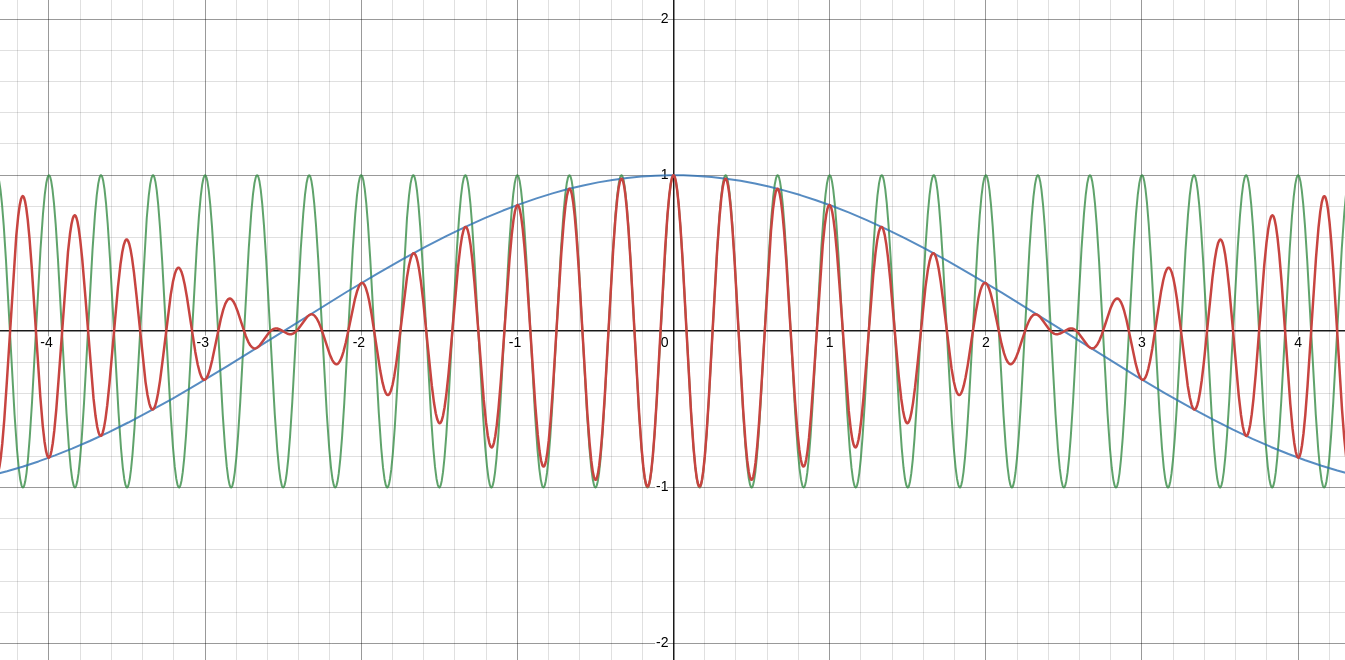
\includegraphics[width=0.48\textwidth]{fig/part-1/ex SA - 11.png}
	\hfill
	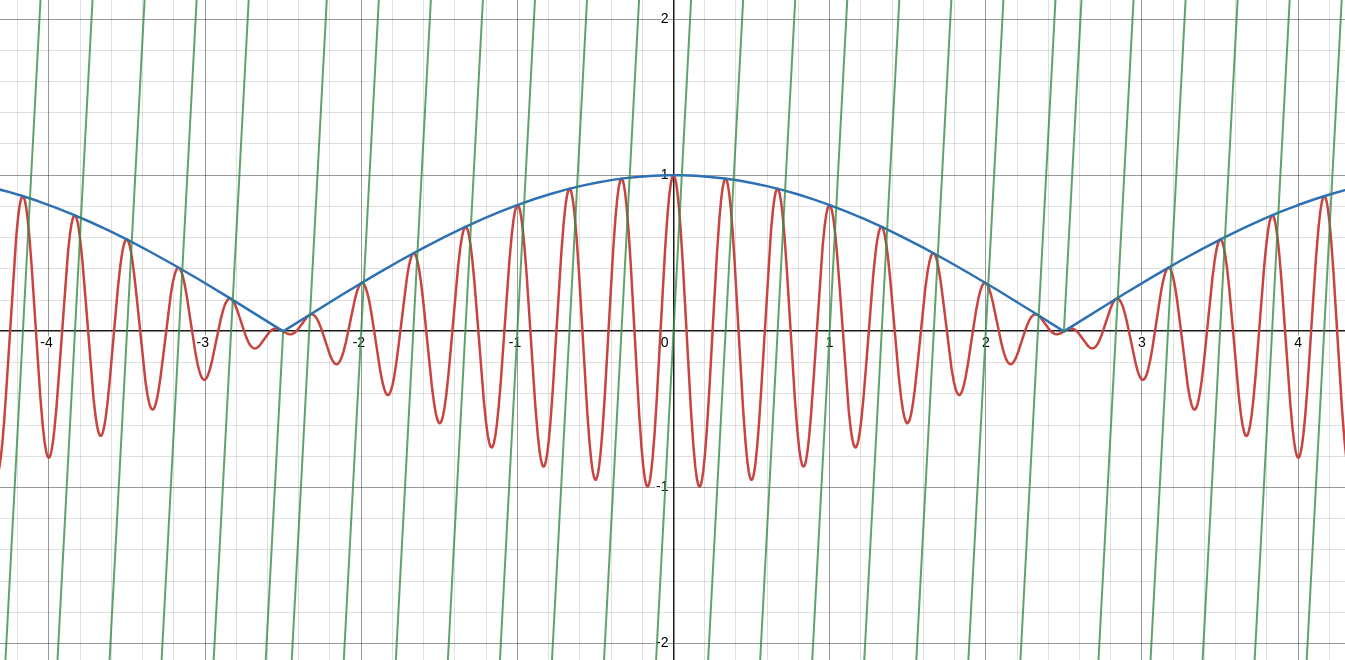
\includegraphics[width=0.48\textwidth]{fig/part-1/ex SA - 12.png}
	\caption[\DONE Décomposition en signal analytique d'un produit de cosinus]{Représentation graphique du signal $x$ (rouge) avec $\nu_1=3$ et $\nu_2=0.1$. Sur l'image de gauche, avec signaux de fréquences pures (bleu et vert). Sur l'image de droite, avec son amplitude (bleu) et sa phase instantanée (vert). Les discontinuités de la phase sont dû à l'arrondi à $2\pi$  près de l'argument de $\SA{x_1}$ et à la façon dont il est calculé lorsque le signal s'annule (mise à 0). Voir \href{https://www.desmos.com/calculator/gcedcdfkhr}{ici} pour un graphique dynamique.}
	\label{fig:exemple_tSA_1/2}
\end{figure}

\noindent
On montre sans mal\footnote{\itshape
	$\fou{x}_1$ est donné par 4 Diracs, en ne gardant que ce non nul sur $\R^+$ on obtient le spectre de $\SA{x_1}$ et il reste plus qu'à inverser la transformée de Fourier.}
que si $\ \nu_1\geq\nu_2$, alors la transformée en SA de $x_1$ s'écrit :
\[\SA{x_1} = \cos \left(2\pi\nu_2 t\right) e^{2i \pi\nu_1 t}\]
\\
Le signal $\SA{x_1}$ n'est ici pas sous forme exponentielle à proprement parler puisque le cosinus peut être négatif et pour s'y ramener, il suffit de passer le cos en valeur absolue et d'ajouter $\pi$ à l'argument lorsque nécessaire. L’avantage de cette forme est qu'elle fait clairement apparaître les fréquences $\nu_{1,2}$. En particulier, la fréquence instantanée du signal est la plus grandes des deux fréquences $\nu_1$ et $\nu_2$. La plus petite, elle, se retrouve dans l'amplitude. 
\\
Ce résultat est rassurant en cela qu'il est plus naturel de voir le cosinus de basse fréquence comme modulant celui de haute fréquence que l'inverse, comme mies en évidence par le premier graphique \Cref{fig:exemple_tSA_1/2}. 
\\
Aussi, en mettant les hautes fréquences du signal dans la fréquence instantanée, on s'assure de limiter les variations de l'amplitude. Cela apporte bien plus de contrainte en terme de décomposition $(a_{x_1},\phi_{x_1})$, en cela qui si l'inverse étant vrai, alors toute les fréquences pourrait être envoyé dans l'amplitude, ce qui laisserait la phase invariante.
\\

Cela étant dit, lorsque l'on fait varier $\nu_1$ et $\nu_2$, le résultat n'est pas toujours si intuitif. C'est notamment le cas lorsque les deux deviennent de plus en plus proche :

\begin{figure}[h]\centering
	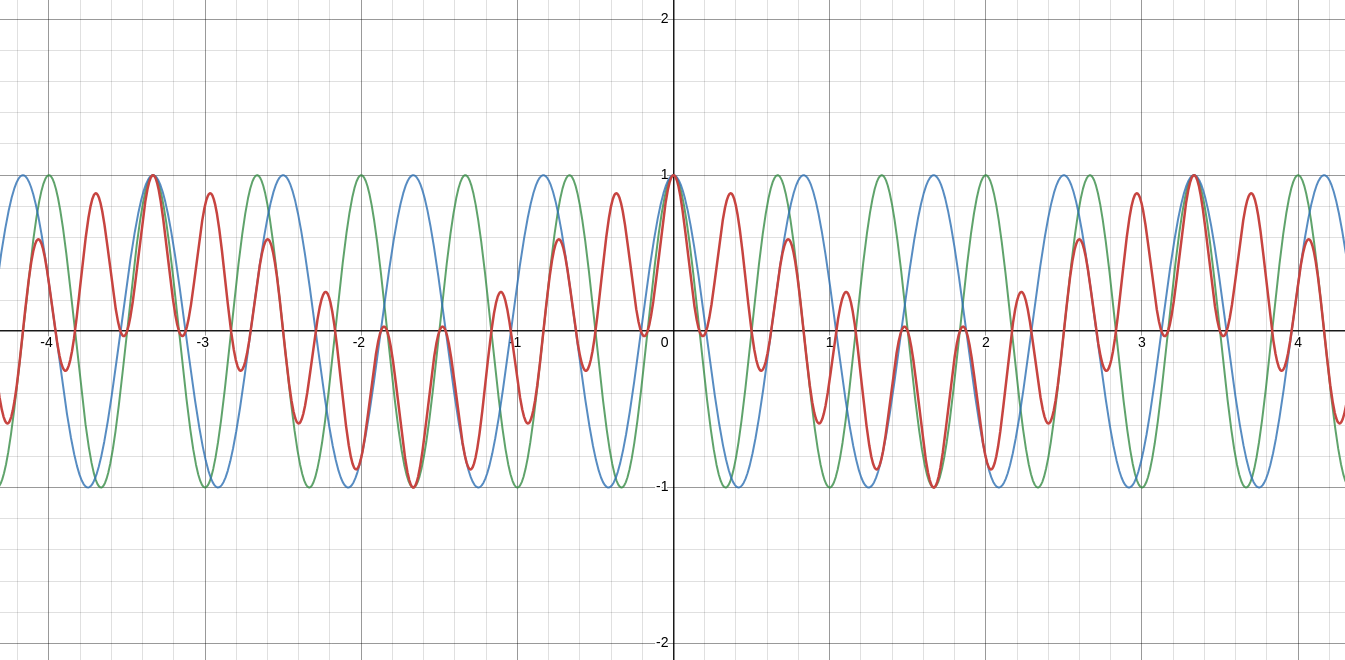
\includegraphics[width=0.48\textwidth]{fig/part-1/ex SA - 21.png}
		\hfill
	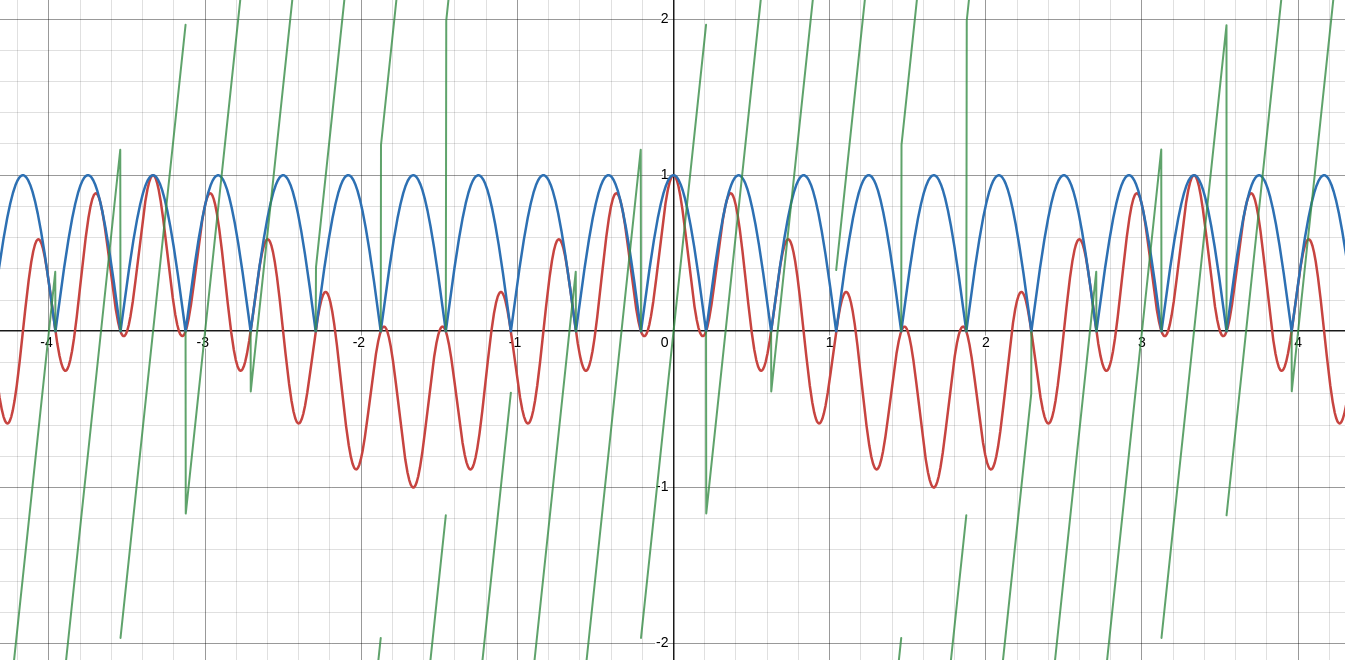
\includegraphics[width=0.48\textwidth]{fig/part-1/ex SA - 22.png}
	\caption{\DONE Idem que pour la figure \ref{fig:exemple_tSA_1/2} précédente, avec cette fois $\nu_1=1.5$ et $\nu_2=1.3$.}
	\label{fig:exemple_tSA_2/2}
\end{figure}

Pour comprendre pourquoi l'amplitude ne fait pas ce qu'on attendrait d'elle, est introduit le théorème de Bedrosian :

\begin{theoreme}[de Bedrosian]\label{theo:2Bedrosian}
	Dans sa formulation la plus générale, le théorème de Bedrosian énonce que si deux fonctions $f,g\in L^2(\R)$ sont telles l'une des trois assertions suivantes est vraie :
	\begin{itemize}%[label=\textit{\arabic*}. ]
		\item 
		\item $\exists \lambda\in\R^+\ |\ \supp \fou{f} \subset [-\lambda, +\infty[,\ \supp \fou{g} \subset [\lambda, +\infty[$\label{item:1condi_theo2Bedrosian}
		
		\item $\exists \lambda\in\R^+\ |\ \supp \fou{f} \subset ]-\infty, \lambda],\ \supp \fou{g} \subset ]-\infty,-\lambda]$ \label{item:2condi_theo2Bedrosian}
		
		\item $\exists (\lambda_1,\lambda_2)\in \R^+\times\R^+ \setminus\{(0,0)\}\ |\ \supp \fou{f} \subset [-\lambda_1, \lambda_2],\ \supp \fou{g} \subset \R\setminus[-\lambda_2,\lambda_1]$
		
	\end{itemize}
	alors la transformée de Hilbert de leur produit s'écrit (voir \cite{wang_simple_2009} pour une démonstration) :
	\begin{equation}\label{eq:2Bedrosian}
		\hilb{fg} = f\hilb{g}
	\end{equation}
\end{theoreme}

Dans le cas d'un signal réel, suivant la \cref{def:ampli-phase_instant} on peut écrire $\ x=a_x\cos \phi_x$.
Comme $a_x$ et $\cos \phi_x$ sont réelles, seule la troisième condition du théorème de Bedrosian peut être satisfaite pour peu que $\lambda_1=\lambda_2$. Ainsi :

\begin{corollaire}\label{coro:AM-FM}
	Toujours avec les même notations, si $a_x\in L^2(\R)$, $\cos\phi_x\in L^2(\R)$ et qu'il existe $\lambda\in\R^{+_*}$ tel que :
	\begin{equation}\label{eq:condiBedro_AM-FM}
		\supp \Fou{a_x} \subset [-\lambda, \lambda],\quad \supp \Fou{\cos\phi_x} \subset \R\setminus[-\lambda,\lambda]
	\end{equation}
	Alors on a :
	\begin{align}\label{eq:result_AM-FM}
		\hilb{x} &= a_x\hilb{\cos \phi_x}  &  \qquad\qquad&\text{et si }a_x(t)\neq 0,  &  \hilb{\cos \phi_x}(t) = \sin\phi_x(t)
	\end{align}
\end{corollaire}
\skipl

Pour interpréter ce \namecref{coro:AM-FM}, prenons un autre exemple : $\ x_2(t) = a(t)\cos(2\pi \nu_0 t)$. Sa transformé de Fourier est donnée par :
\begin{align*}
	\fou{x}_2(\nu) &= \fou{a}(\nu)*\frac{1}{2}\Big(\delta(\nu-\nu_0) + \delta(\nu+\nu_0)\Big) \\
	&= \frac{1}{2}\Big(\fou{a}(\nu+\nu_0) + \fou{a}(\nu-\nu_0)\Big)
\end{align*}
\\
Graphiquement, la transformé de Fourier de $x_2$ duplique le graphe de $\fou{a}$ en $\pm\nu_0$ et somme les deux. La condition \eqref{eq:condiBedro_AM-FM} du \cref{coro:AM-FM} demande alors que $\nu_0$ soit choisie de telle sorte que :
\[\supp \Fou{a}\subset[-\nu_0, \nu_0]\]
\\
C'est-à-dire qu'il n'y ait pas de chevauchement entre les deux courbes $\ \Gamma_\pm : \nu \longmapsto \fou{a}(\nu\mp\nu_0) $ (voir \cref{fig:alising-ish} ci-dessous). Moralement, cela assure qu'en ne prenant que la partie positive du spectre de $x_2$, l'on ne ramène pas avec une partie de $\fou{a}(\nu+\nu_0)$. Quant bien même cette explication est simpliste puisqu'ici $\phi$ est linaire, on peut voir que le phénomène est finalement très proche de celui d'aliasing.
\\

\begin{figure}[h]\centering
	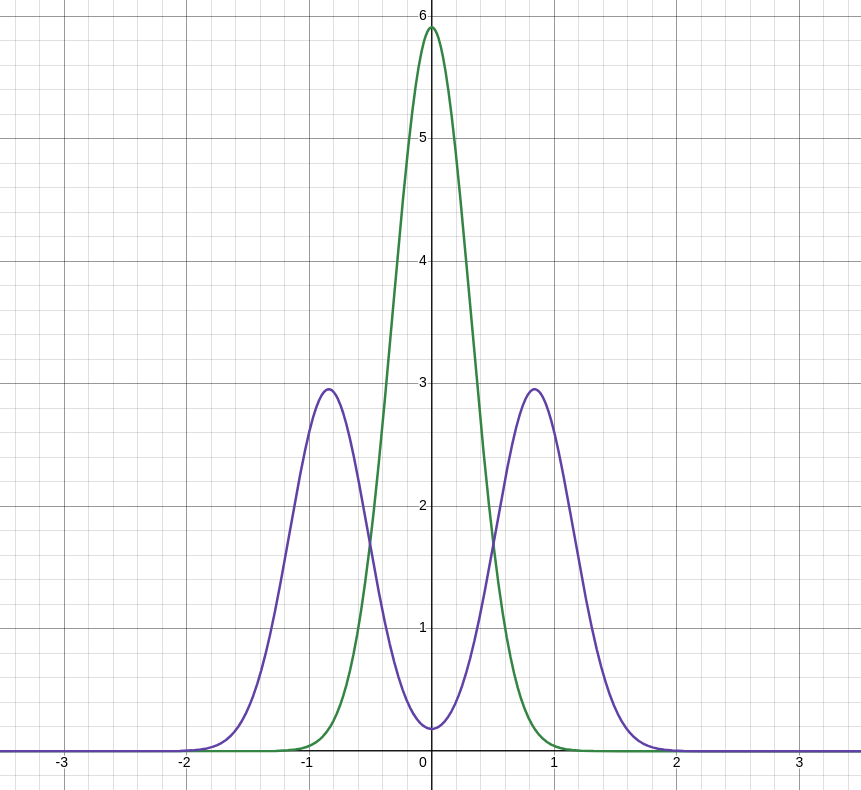
\includegraphics[width=0.45\textwidth]{fig/part-1/bedro condi 1.png} 
	\hfill
	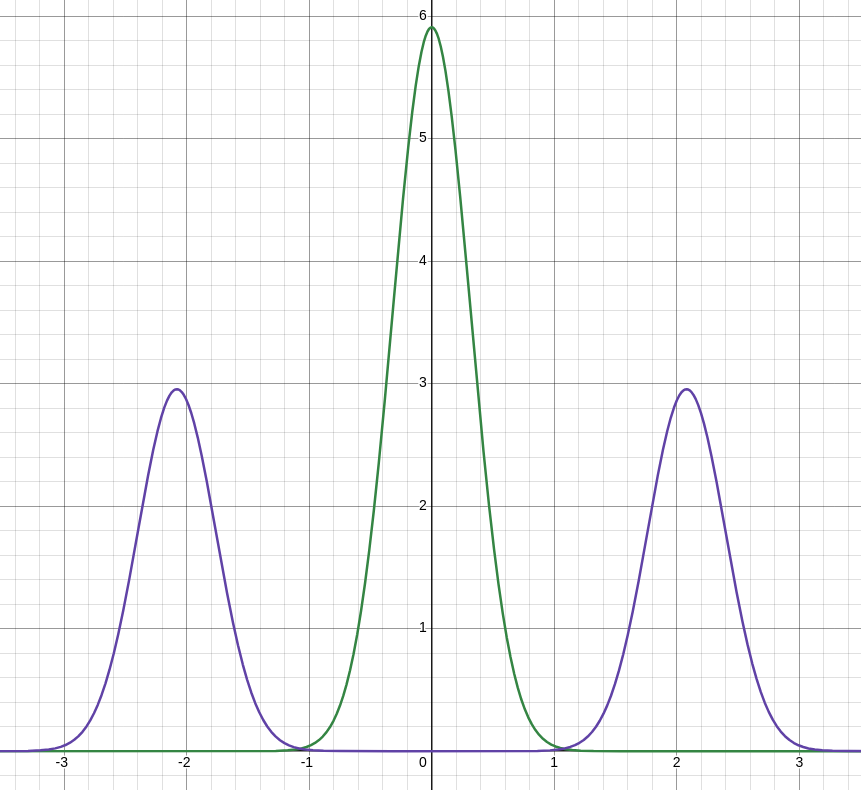
\includegraphics[width=0.45\textwidth]{fig/part-1/bedro condi 2.png} 
	\caption[\DONE Représentation de l'hypothèse du Théorème de Bedrosian]{Sur les deux graphiques sont représentés en vert $\fou{a}$ et en violet $\fou{x}_2$. Dans le premier cas l'hypothèse de Bedrosian et respectée mais pas dans le second.}
	\label{fig:alising-ish}
\end{figure}


Pour revenir sur l'exemple $x_1$ précédent, dans la seconde figure \ref{fig:exemple_tSA_2/2}, l'amplitude ne colle plus à l'interprétation que l'on voudrait justement parce que la condition de Bedrosian n'est plus respecter (à savoir $\nu_1\geq 2\nu_2$). 




\subsection{Démonstrations de la \cref{prop:phases_2var}}\label{ann:demo_phases_2var}

\subsubsection{Formule de la phase totale \eqref{eq:phaset_2var}}

On note $\mathcal{V} = \begin{pmatrix} \cos\chi \\ -i\sin\chi \end{pmatrix}$ et on a :
\begin{align*}
	\phaset{\x} = \big\langle \x(t), \x(t_0)\big\rangle &= \Big\langle a(t)e^{\i \varphi(t)}R_{\theta(t)}\mathcal{V}(t), a(t_0)e^{\i \varphi(t_0)}R_{\theta(t_0)}\mathcal{V}(t_0) \Big\rangle \\
	&= a(t)e^{\i \varphi(t)} a(t_0)e^{-\i \varphi(t_0)} \Big\langle R_{\theta(t)}\mathcal{V}(t), R_{\theta(t_0)}\mathcal{V}(t_0) \Big\rangle \\
	%&= a(t_0)a(t)e^{\i (\varphi(t_0)-\varphi(t))}\Big\langle \mathcal{V}(t_0), R_{\theta(t_0)}^{-1}R_{\theta(t)}\mathcal{V}(t) \Big\rangle \\
	&= a(t_0)a(t)e^{\i (\varphi(t)-\varphi(t_0))}\Big\langle R_{\theta(t)- \theta(t_0)}\mathcal{V}(t), \mathcal{V}(t_0) \Big\rangle
\end{align*}
Pour alléger les notations, on note $\ \Delta y =y(t)-y(t_0)$, $\ y_1=y(t_0)\ $ et $\ y_2=(t)\ $ pour $\ y=\varphi,\theta,\chi$. Le produit hermitien à droite s'écrit alors :
\begin{align*}
	\Big\langle R_{\Delta\theta}\mathcal{V}(t), \mathcal{V}(t_0) \Big\rangle &=   \Big(\cos\Delta\theta \cos\chi_2 + i\sin\Delta\theta \sin\chi_2 \qquad \sin\Delta\theta \cos\chi_2 - i\cos\Delta\theta \sin\chi_2\Big) \begin{pmatrix} \cos\chi_1 \\ i\sin\chi_1 \end{pmatrix} \\
	&= \cos\chi_1\Big(\cos\Delta\theta \cos\chi_2 + i\sin\Delta\theta \sin\chi_2\Big) + i\sin\chi_1\Big(\sin\Delta\theta \cos\chi_2 - i\cos\Delta\theta \sin\chi_2\Big) \\
	&= \cos\Delta\theta \Big(\cos\chi_1 \cos\chi_2 + \sin\chi_1 \sin\chi_2\Big) + i\sin\Delta\theta \Big( \cos\chi_1 \sin\chi_2 + \sin\chi_1\cos\chi_2\Big) \\
	&= \cos\Delta\theta \cos\Delta\chi + i\sin\Delta\theta \sin(\chi_1+\chi_2)
\end{align*}
\\
D'où la phase totale :
\begin{align*}
	\phaset(\x) = \arg\big\langle \x(t), \x(t_0)\big\rangle &= \arg\left( a(t_0)a(t)e^{\i (\varphi(t) - \varphi(t_0))}\Big( \cos\Delta\theta \cos\Delta\chi + i\sin\Delta\theta \sin(\chi_1+\chi_2) \Big) \right) \\
	&= \varphi(t) - \varphi(t_0) + \arg\Big( \cos\Delta\theta \cos\Delta\chi + i\sin\Delta\theta \sin(\chi_1+\chi_2) \Big)
\end{align*}
et l'argument restant s'écrit comme une arctangente, donnant :
\begin{align*}
	\phaset(\x) &= \varphi(t)-\varphi(t_0) + \arctan\frac{\sin\Delta\theta \sin(\chi_1+\chi_2)}{\cos\Delta\theta \cos\Delta\chi} \\
	&= \varphi(t)-\varphi(t_0) + \arctan \left( \tan\Delta\theta\frac{\sin(\chi_1+\chi_2)}{\cos\Delta\chi} \right) \\
	&= \cdots
\end{align*}
\skipl




\subsubsection{Formule de la phase dynamique \eqref{eq:phased_2var}}

Par souci de lisibilité, on note $\ \mathcal{U} = R_{\theta} \begin{pmatrix} \cos\chi \\ -i\sin\chi \end{pmatrix} = \begin{pmatrix} \cos\theta(t) \cos\chi(t) + i\sin\theta(t) \sin\chi(t) \\ \sin\theta(t) \cos\chi(t) - i\cos\theta(t) \sin\chi(t) \end{pmatrix}$, de sorte que la dérivée de $\ \x=ae^{\i \varphi}\mathcal{U}\ $ s'écrive :
\[\dot{\x} = a'e^{\i \varphi}\mathcal{U} + ia\varphi'e^{\i \varphi} \mathcal{U} + ae^{\i \varphi}\theta'\begin{pmatrix} -\sin\theta \cos\chi + i\cos\theta \sin\chi \\ \cos\theta \cos\chi + i\sin\theta \sin\chi \end{pmatrix} + ae^{\i \varphi}\chi'\begin{pmatrix} -\cos\theta \sin\chi + i\sin\theta \cos\chi \\ -\sin\theta \sin\chi - i\cos\theta \cos\chi \end{pmatrix}\]
\\
Les vecteurs des deux derniers membres s'expriment en fonction des composantes $\ \mathcal{U}_{1,2}\ $ de $\ \mathcal{U}$ :
\begin{align*}
	\begin{pmatrix} -\sin\theta \cos\chi + i\cos\theta \sin\chi \\ \cos\theta \cos\chi + i\sin\theta \sin\chi \end{pmatrix} &= \begin{pmatrix} -\mathcal{U}_2 \\ \mathcal{U}_1 \end{pmatrix}  &
	\begin{pmatrix} -\cos\theta \sin\chi + i\sin\theta \cos\chi \\ -\sin\theta \sin\chi - i\cos\theta \cos\chi \end{pmatrix} &= i\begin{pmatrix} \congu{\mathcal{U}}_2 \\ -\congu{\mathcal{U}}_1 \end{pmatrix}
\end{align*}
\\
Le produit hermitien $\langle \dot{\x}, \x \rangle$ s'écrit alors :
\begin{align*}
	\langle \dot{\x}, \x \rangle 
	&= \left\langle a'e^{\i \varphi}\mathcal{U} + ia\varphi'e^{\i \varphi} \mathcal{U} + ae^{\i \varphi}\theta'\begin{pmatrix} -\mathcal{U}_2 \\ \mathcal{U}_1 \end{pmatrix} + iae^{\i \varphi}\chi'\begin{pmatrix} \congu{\mathcal{U}}_2 \\ -\congu{\mathcal{U}}_1 \end{pmatrix}, ae^{\i \varphi}\mathcal{U} \right\rangle \\
	&= \left\langle a'\mathcal{U} + ia\varphi' \mathcal{U} + a\theta'\begin{pmatrix} -\mathcal{U}_2 \\ \mathcal{U}_1 \end{pmatrix} + ia\chi'\begin{pmatrix} \congu{\mathcal{U}}_2 \\ -\congu{\mathcal{U}}_1 \end{pmatrix}, a\mathcal{U} \right\rangle \\
	&= aa' \big\langle \mathcal{U}, \mathcal{U}\big\rangle  + ia^2\varphi' \big\langle \mathcal{U}, \mathcal{U}\big\rangle  + a^2\theta'\left\langle \begin{pmatrix} -\mathcal{U}_2 \\ \mathcal{U}_1 \end{pmatrix}, \mathcal{U} \right\rangle + ia^2\chi'\left\langle \begin{pmatrix} \congu{\mathcal{U}}_2 \\ -\congu{\mathcal{U}}_1 \end{pmatrix}, \mathcal{U} \right\rangle
\end{align*}
où les deux derniers termes donnent :
\begin{align*}
	\left\langle \begin{pmatrix} -\mathcal{U}_2 \\ \mathcal{U}_1 \end{pmatrix}, \mathcal{U} \right\rangle &= -\mathcal{U}_2\congu{\mathcal{U}}_1 + \mathcal{U}_1\congu{\mathcal{U}}_2 \\
	&= 2i\Im m\big(\mathcal{U}_1 \congu{\mathcal{U}}_2\big) \\
	&= 2i\Im m\Big(\big( \cos\theta \cos\chi + i \sin\theta \sin\chi \big) \big( \sin\theta \cos\chi + i \cos\theta \sin\chi \big)\Big) \\
	&= 2i\big(\cos^2\theta \cos\chi \sin\chi + \sin^2\theta \sin\chi \cos\chi \big) \\
	&= 2i \cos\chi \sin\chi \\
	&= i\sin2\chi 
	\\ \\
	\left\langle \begin{pmatrix} \congu{\mathcal{U}}_2 \\ -\congu{\mathcal{U}}_1 \end{pmatrix}, \mathcal{U} \right\rangle &= \congu{\mathcal{U}_2\mathcal{U}_1} - \congu{\mathcal{U}_1\mathcal{U}_2} = 0
\end{align*}
\skipl

D'où, sachant que $\ \|\x\|^2=a^2\ $ et $\ \|\mathcal{U}\|=1$, la formule :
\begin{align*}
	\frac{\Im m\big\langle \dot{\x}, \x\big\rangle}{\|\x\|^2} &= \frac{1}{a^2}\Im m\Big(aa' \big\langle \mathcal{U}, \mathcal{U}\big\rangle  + ia^2\varphi' \big\langle \mathcal{U}, \mathcal{U}\big\rangle + ia^2\theta' \sin2\chi \Big) \\
	&= \frac{1}{a^2} \Big( a^2\varphi' \|\mathcal{U}\|^2 + a^2\theta' \sin2\chi \Big) \\
	&= \varphi' + \theta' \sin2\chi
\end{align*}